% vim: foldmethod=marker foldlevel=0

% -----------------------------------------------------------------------------
% unusual(?) dependencies
% -----------------------------------------------------------------------------
%
% - minted: version 2+
% - Pygments: for the minted package


% -----------------------------------------------------------------------------
% information
% -----------------------------------------------------------------------------

\def \docAuthor {Ben Blazak}
\def \docClass  {CPSC 120 SI}
\def \docSchool {California State University Fullerton}
\def \docTerm   {Fall 2014}
\def \docTitle  {Week 5 Worksheet}


% -----------------------------------------------------------------------------
% document setup
% -----------------------------------------------------------------------------
% {{{

\documentclass[12pt,letterpaper]{article}

\usepackage[includehead,
            includefoot,
            margin=1in,
            top=.25in,
            headheight=.75in,
            headsep=.25in,
            footskip=.25in,
           ]{geometry}

\usepackage[fleqn]{amsmath}
\usepackage{amssymb}
\usepackage{array}
\usepackage[shortlabels]{enumitem}
\usepackage{fancybox}
\usepackage{fancyhdr}
\usepackage{l3regex}
\usepackage{luacode}
\usepackage{mathtools}
\usepackage[framemethod=TikZ]{mdframed}
\usepackage{minted}
\usepackage{multicol}
\usepackage{multirow}
\usepackage{tikz}
\usepackage[normalem]{ulem}
\usepackage{url}
\usepackage{xcolor}


% text ------------------------------------------------------------------------

\binoppenalty = 10000  % never break next to a binary operator
\relpenalty   = 10000  % never break next to a relation operator

\setlength{\parindent}{0em}
\setlength{\parskip}{1ex}

\setlist[itemize]{nosep,itemsep=.5ex,parsep=.5ex}

% math ------------------------------------------------------------------------

\setlength{\mathindent}{1cm}

% - "\begin{document}" resets these values, so they have to be treated
%   specially
\AtBeginDocument{
  \setlength{\abovedisplayskip}{1.5ex plus .5ex minus .5ex}
  \setlength{\belowdisplayskip}{1.5ex plus .5ex minus .5ex}
}

% source code -----------------------------------------------------------------

\usemintedstyle{solarizedlight}

% header and footer -----------------------------------------------------------

\pagestyle{fancy}

\lhead{\docClass}
\rhead{\docTitle}
\cfoot{\thepage}
\renewcommand{\headrule}{\hrule height 0.4pt}
\renewcommand{\footrule}{\hrule height 0.4pt}

\fancypagestyle{firstpage}{
  \fancyhead[L]{\docAuthor\\\docClass}
  \fancyhead[C]{\docSchool\\}
  \fancyhead[R]{\docTerm\\\docTitle}
}


% -----------------------------------------------------------------------------
% macros
% -----------------------------------------------------------------------------

% abbreviations ---------------------------------------------------------------

\def \<{\langle}
\def \>{\rangle}

\def \ε{\varepisilon}
\def \θ{\vartheta}
\def \κ{\varkappa}
\def \π{\varpi}
\def \ρ{\varrho}
\def \σ{\varsigma}
\def \φ{\varphi}

\def \Γ{\varGamma}
\def \Δ{\varDelta}
\def \Θ{\varTheta}
\def \Λ{\varLambda}
\def \Ξ{\varXi}
\def \Π{\varPi}
\def \Σ{\varSigma}
\def \Υ{\varUpsilon}
\def \Φ{\varPhi}
\def \Ψ{\varPsi}
\def \Ω{\varOmega}

% special characters ----------------------------------------------------------

\catcode `α = \active \let α \alpha
\catcode `β = \active \let β \beta
\catcode `γ = \active \let γ \gamma
\catcode `δ = \active \let δ \delta
\catcode `ε = \active \let ε \epsilon
\catcode `ζ = \active \let ζ \zeta
\catcode `η = \active \let η \eta
\catcode `θ = \active \let θ \theta
\catcode `ι = \active \let ι \iota
\catcode `κ = \active \let κ \kappa
\catcode `λ = \active \let λ \lambda
\catcode `μ = \active \let μ \mu
\catcode `ν = \active \let ν \nu
\catcode `ξ = \active \let ξ \xi
\catcode `ο = \active \let ο o
\catcode `π = \active \let π \pi
\catcode `ρ = \active \let ρ \rho
\catcode `σ = \active \let σ \sigma
\catcode `τ = \active \let τ \tau
\catcode `υ = \active \let υ \upsilon
\catcode `φ = \active \let φ \phi
\catcode `χ = \active \let χ \chi
\catcode `ψ = \active \let ψ \psi
\catcode `ω = \active \let ω \omega

\catcode `Α = \active \let Α A
\catcode `Β = \active \let Β B
\catcode `Γ = \active \let Γ \Gamma
\catcode `Δ = \active \let Δ \Delta
\catcode `Ε = \active \let Ε E
\catcode `Ζ = \active \let Ζ Z
\catcode `Η = \active \let Η H
\catcode `Θ = \active \let Θ \Theta
\catcode `Ι = \active \let Ι I
\catcode `Κ = \active \let Κ K
\catcode `Λ = \active \let Λ \Lambda
\catcode `Μ = \active \let Μ M
\catcode `Ν = \active \let Ν N
\catcode `Ξ = \active \let Ξ \Xi
\catcode `Ο = \active \let Ο O
\catcode `Π = \active \let Π \Pi
\catcode `Ρ = \active \let Ρ P
\catcode `Σ = \active \let Σ \Sigma
\catcode `Τ = \active \let Τ T
\catcode `Υ = \active \let Υ \Upsilon
\catcode `Φ = \active \let Φ \Phi
\catcode `Χ = \active \let Χ X
\catcode `Ψ = \active \let Ψ \Psi
\catcode `Ω = \active \let Ω \Omega

% functions -------------------------------------------------------------------

\def \ceil #1{\left\lceil#1\right\rceil}
\def \floor #1{\left\lfloor#1\right\rfloor}

% }}}
% other -----------------------------------------------------------------------
% {{{

% - sometimes a "\par", especially at the end of a block, is necessary to
%   prevent an extra (empty) paragraph from appearing in the output
% - `\color{.!50}` means 50 percent of the current color

     \def \note     #1{{\color{.!50}#1\par}}
\long\def \longnote #1{{\color{.!50}#1\par}}

\long\def \subquestion #1{
  \par #1 \par
}
\long\def \subproof #1{
  \vspace{1ex}\par\textbf{\textit{Proof.}} #1 \unskip\hfill$\square$\par\vspace{1ex}
}
\long\def \subsolution #1{
  \vspace{1ex}\par\textbf{\textit{Solution.}} #1 \unskip\hfill$\square$\par\vspace{1ex}
}

\long\def \question #1{\filbreak\subquestion{#1}}
\long\def \proof    #1{\subproof{#1}}
\long\def \solution #1{\subsolution{#1}}

\def \inputcppwithsol #1{
  \vspace{1.5ex}
  \begin{mdframed}[roundcorner=3mm,backgroundcolor=black!5]
    \centering \luaexec{tex.print((string.gsub('#1','_','\\_')))}
  \end{mdframed}
  \vspace{-4ex}
  \inputminted{cpp}{#1}
  \inputminted[frame=single,rulecolor=\color{.!30},framesep=2mm]{text}
              {#1.txt}
}  

% }}}
% -----------------------------------------------------------------------------
% document
% -----------------------------------------------------------------------------

% rough overview of topics for this week
% . syntax and stuff
%   . declaration vs initialization
%   . math library
%   . operators
%   . cin and cout
%     - input errors
% . data types
%   . integer division
%   . the dangers of float
%   . typecasting and promotion
% . practice
%   . equivalent declarations and assignments
%   . converting algebra into c++
%   . order of operations and associativity
%   . 'a'+5
% - program design!

\begin{document}
\thispagestyle{firstpage}

The website for these SI sessions is
\url{https://github.com/benblazak/2014-fall-si-cpsc120}.

Many of these examples are from
\url{https://github.com/benblazak/2014-spring-si-cpsc120}, which is full of
stuff I wrote for a lab last semester.  If you're looking for extra practice,
this is one of many places you might start.

Along with your book, \url{http://www.cplusplus.com/doc/tutorial/} is a great
resource for tutorials, and \url{http://www.cplusplus.com/reference/clibrary/}
is a great reference.


\filbreak
\section*{Syntax and Stuff}
\begin{itemize}[itemsep=10ex]

  \item What's the difference between the ``declaration'' and the
    ``initialization'' of a variable?

  \item What is the \mintinline{cpp}{cmath} library?  Where can I learn about
    it?

  \item What is a binary operator?  A unary operator?

  \item What is operator precedence?  Associativity?

  \item What is the syntax for a \mintinline{cpp}{cout} statement (i.e.~what
    are each of the pieces in a full statement beginning with
    \mintinline{cpp}{cout})?

  \item What is the syntax for a \mintinline{cpp}{cin} statement?

\end{itemize}


\filbreak
\section*{Practice}
\begin{itemize}[itemsep=15ex]

  \item At the beginning of your program, you want a variable
    \mintinline{cpp}{a} equal to \mintinline{cpp}{5} and a variable
    \mintinline{cpp}{b} equal to \mintinline{cpp}{7}.  What are three different
    ways to write this?

  \item Convert the following equations to C++ syntax:
    \begin{itemize}[(a),itemsep=7ex]

      \item $c = \sqrt{a^2+b^2}$

      \item $x = \dfrac{-b \pm \sqrt{b^2 - 4ac}}{2a}$

    \end{itemize}
    \vspace{7ex}

\end{itemize}


\filbreak
\section*{Program Design}
From the Abacus International Math Challenge, for Grades 3--4:

\begin{quote}
  A.975. The Strongest Man of Etown had to roll a huge rock ball 10 meters. The
  spectators may guess the weight of the ball. Four people gave the following
  guesses to the organizers: 196 kg, 163 kg, 178 kg, and 185 kg. One guess was
  1 kg off, one was 6 kg off, one was 17 kg off, and one was 16 kg off.  How
  many kg was the weight of the ball?
\end{quote}

How could we find the answer using C++?


\filbreak
\section*{Code}
         \inputcppwithsol{operators.cpp}
\filbreak\inputcppwithsol{float.cpp}
\filbreak\inputcppwithsol{typecast.cpp}


\filbreak
\section*{Things to Think About}
\begin{itemize}

  \item What the heck do \mintinline{cpp}{<<} and \mintinline{cpp}{>>} do in
    the context of input and output streams?  (Note: Looking into this
    thoroughly will take you into the realm of objects, operator overloading,
    and all sorts of fun stuff you won't be seeing in class for a long while.
    Still worth looking into though.)

    \url{http://www.cplusplus.com/reference/ostream/ostream/operator%3C%3C/}

    \url{http://www.cplusplus.com/reference/istream/istream/operator%3E%3E/}

  \item What's a ``stream''?

    \url{http://stackoverflow.com/questions/12145357/c-what-is-a-stream}

    \url{http://www.cprogramming.com/tutorial/c++-iostreams.html}

  \item Why \mintinline{cpp}{static_cast} instead of other types of casting?

    \url{http://stackoverflow.com/questions/103512/in-c-why-use-static-castintx-instead-of-intx}

  \item What is a \mintinline{cpp}{namespace}, and why are they important?

    \url{http://www.cprogramming.com/tutorial/namespaces.html}

\end{itemize}


\filbreak
\section*{Operator Precedence and Associativity List}
From \url{http://www.cplusplus.com/doc/tutorial/operators/} near the bottom of
the page.

\vspace{5ex}

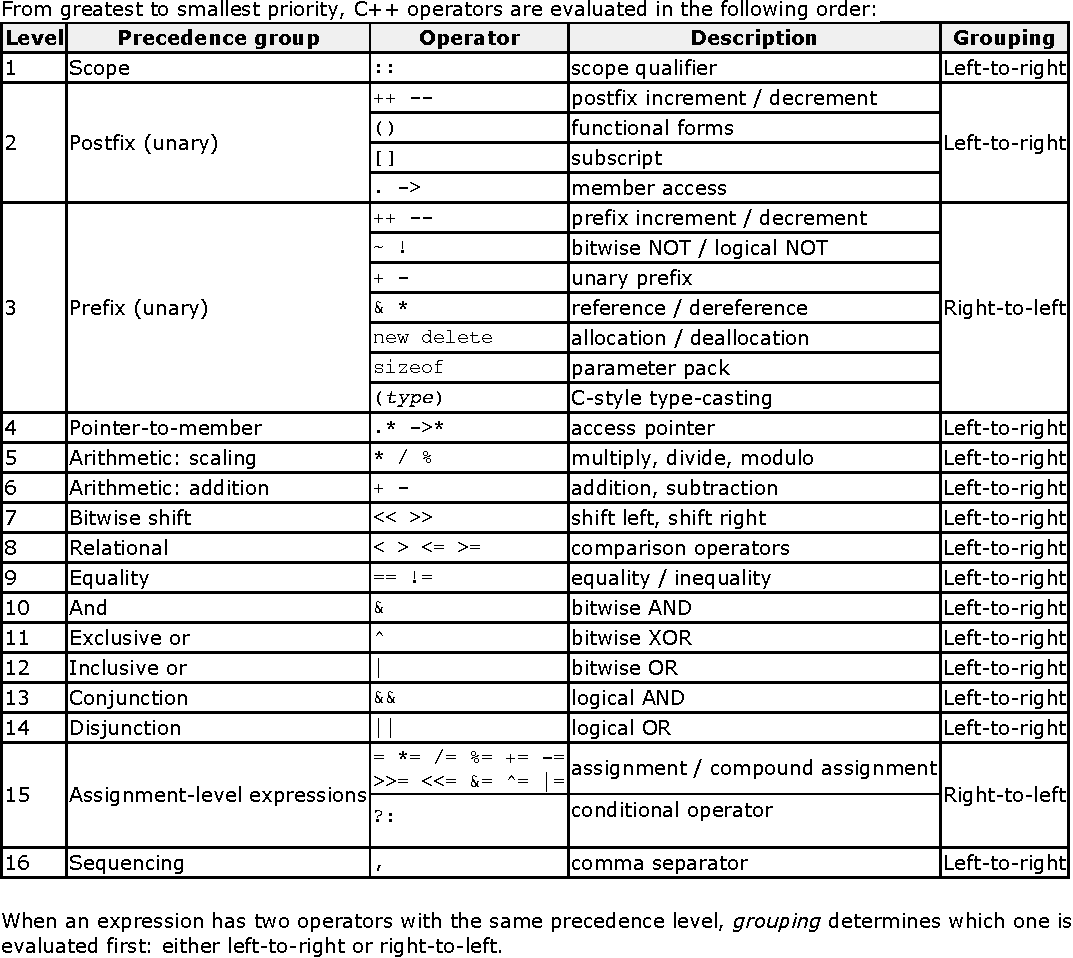
\includegraphics[width=\textwidth]{cplusplusdotcom--operator-prescedence.pdf}


\end{document}

